%<><><><><><><><><><><><><><><><><><><><><><><><><><><><><><><><><><><><><><><><><><><><><>
 % Analysis of existing data
 %<><><><><><><><><><><><><><><><><><><><><><><><><><><><><><><><><><><><><><><><><><><><><>

\section{Analysis of existing data}
We investigated the challenges of reconstructing 2$\pi^0$ final states
with a missing recoil proton using the 2017 GlueX data taken with a
Hydrogen target and the 2019 PrimEx-Eta data with Beryllium and Helium targets.
\subsection{Hydrogen target}
  We selected and reconstructed events that matched the
topology of the reaction $\gamma p\rightarrow \gamma \gamma \gamma
\gamma\, (p)$ with a missing proton. A kinematic fit was performed
that conserved energy and momentum and imposed a vertex constraint at
z=65 cm (CL $> 10^{-6}$). We note that even though the vertex was
fixed at 65 cm to perform the fit, the actual target extends from 50
to 80 cm. Several other nominal selections were imposed to clean up
the event sample, including no charged tracks and no missing
energy. No constraints were imposed on the $\pi^0$ mass in order to
study backgrounds. Accidental background subtractions were performed
to obtain the resulting mass distributions.
\begin{figure}[tph] 
\centering
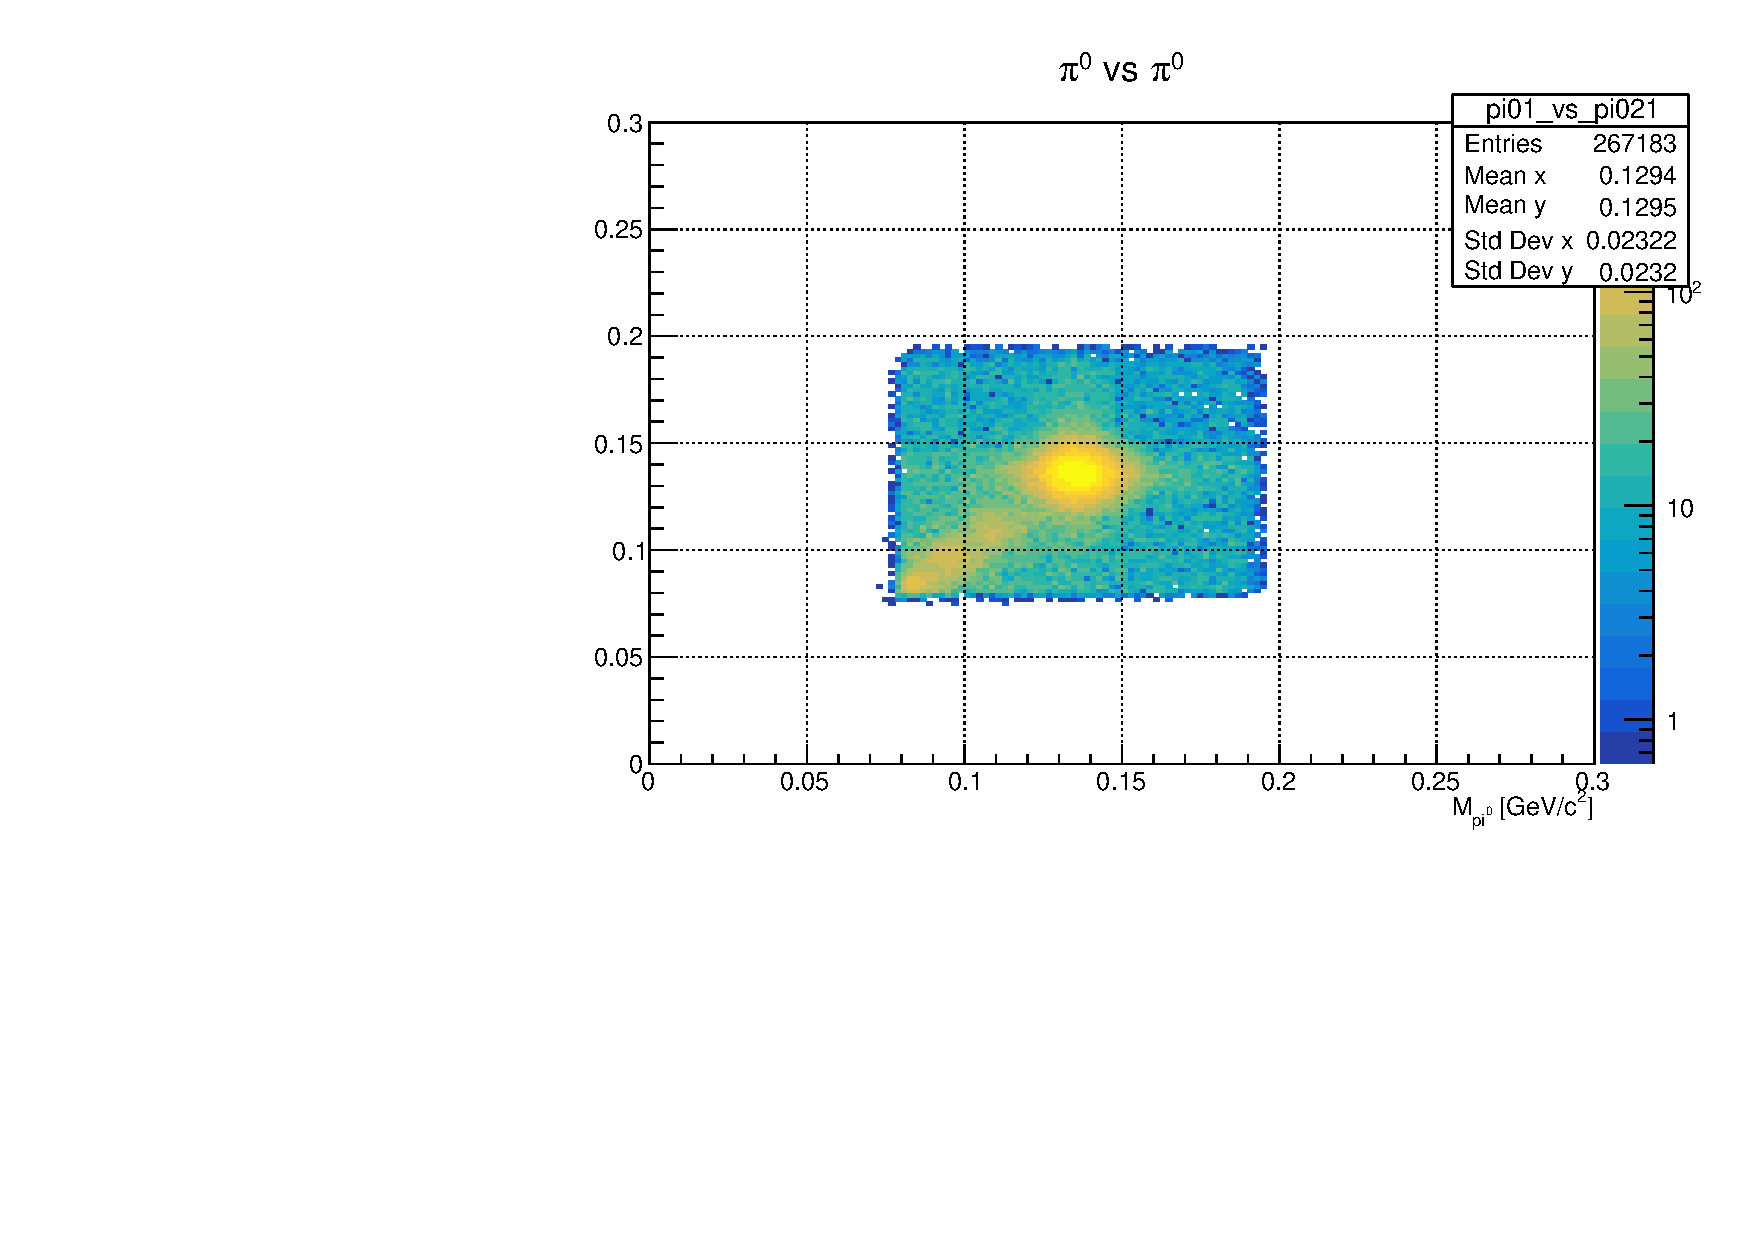
\includegraphics[width=4.75in]{figures/pi0VSpi0.pdf} \\
\centering
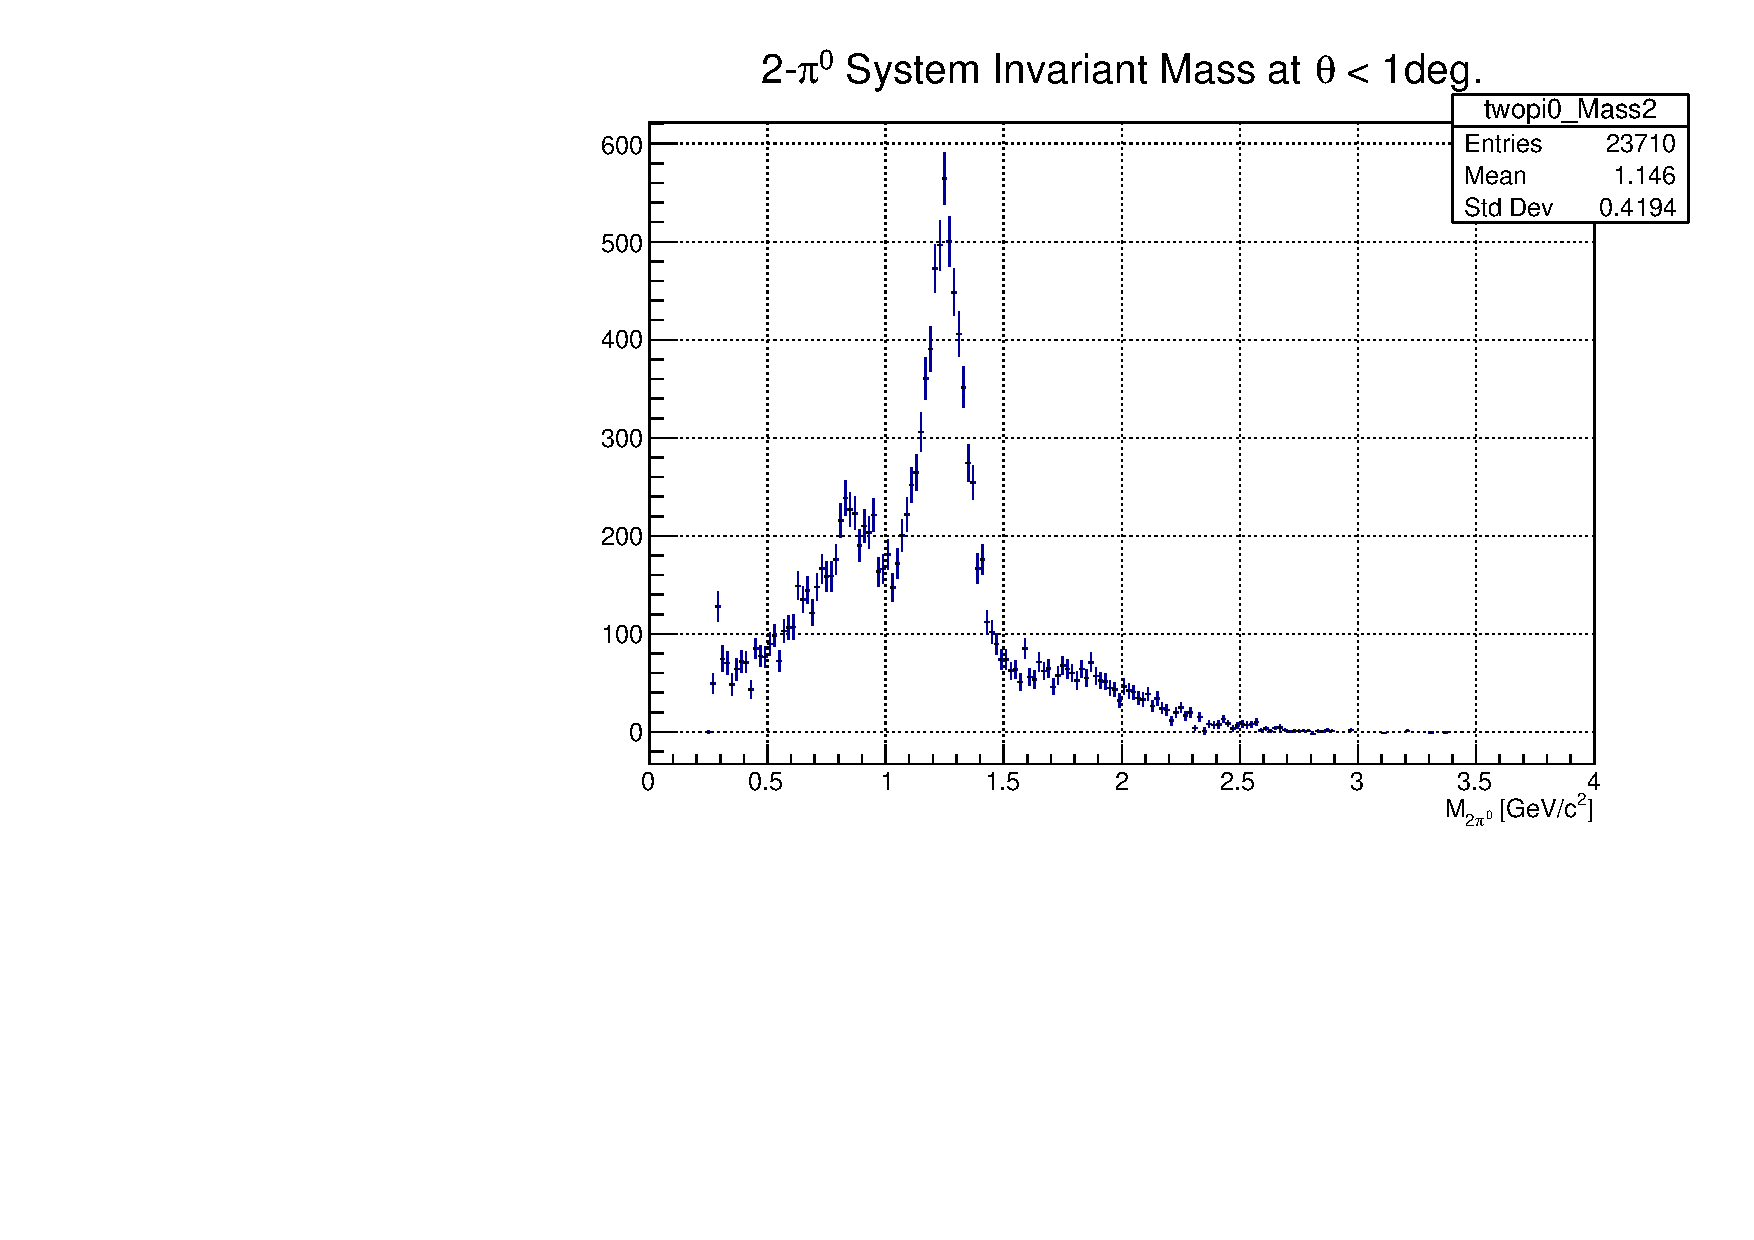
\includegraphics[width=4.75in]{figures/TwoPiInvMass.pdf}
\caption{Experimental distributions from the 2017 GlueX data set analyzed as $\gamma p\rightarrow \gamma \gamma \gamma \gamma\, (p)$ with a missing proton. Top: Two photon invariant mass of one pair vs the two photon invariant mass of the second pair. Bottom: 2$\pi$ mass distribution selecting events with the reconstructed photon pair masses close to the $\pi^0$ mass as  shown above. The plot also requires that the angle of the two pion system be less than 1 degree.
\label{fig:TwoPiInvMass}}
\end{figure}

The invariant mass distributions of two photon pairs each show a
strong $\pi^0$ peak, as shown in the top of
Fig.\,\ref{fig:TwoPiInvMass}. There are background events that fall
under the two $\pi^0$ peaks, which requires further study,
nevertheless, using the selection of photon pairs that reconstruct to
the $\pi^0$, we can plot the 2$\pi^0$ mass spectrum (bottom of
Fig.\,\ref{fig:TwoPiInvMass}). The mass spectrum has recognizable
features, in particular the prominent $f_2(1270)$ that decays to
$\pi^0\pi^0$ 85\% of the time. The structure at $M_{\pi\pi}\sim$0.8
GeV appears too low for the $f_0(980)$ and is present in a location
where the Crystal Ball data \cite{Marsiske:1990hx} shows a low
yield. The yield for $M_{\pi\pi}<$0.5 GeV is consistent within a
factor of two of the relative yield compared to the $f_2(1270$ peak in
the Crystal Ball data. This analysis demonstrates that these neutral
events can be analyzed in our detector under significant more
challenging circumstances than we anticipate for the Primakoff
experiment. In particular, for the Primakoff experiment, we will have
a point nuclear target that will allow valid geometrical constraints
and limit the amount of missing momentum in the reaction. This will
make the kinematic fitting more effective.

It is evident from top plot in fig.~\ref{fig:TwoPiInvMass} that a cut
on the invariant mass of one reconstructed $\pi^{0}$ will reduce the
background on the other $\pi^{0}$ significantly. This is shown in
fig.~\ref{fig:pi0yield} where a cut on the invariant of one $\pi^{0}$
significantly reduces the background in the other while keeping the
main signal mostly undisturbed.
\begin{figure}[htp]
\centering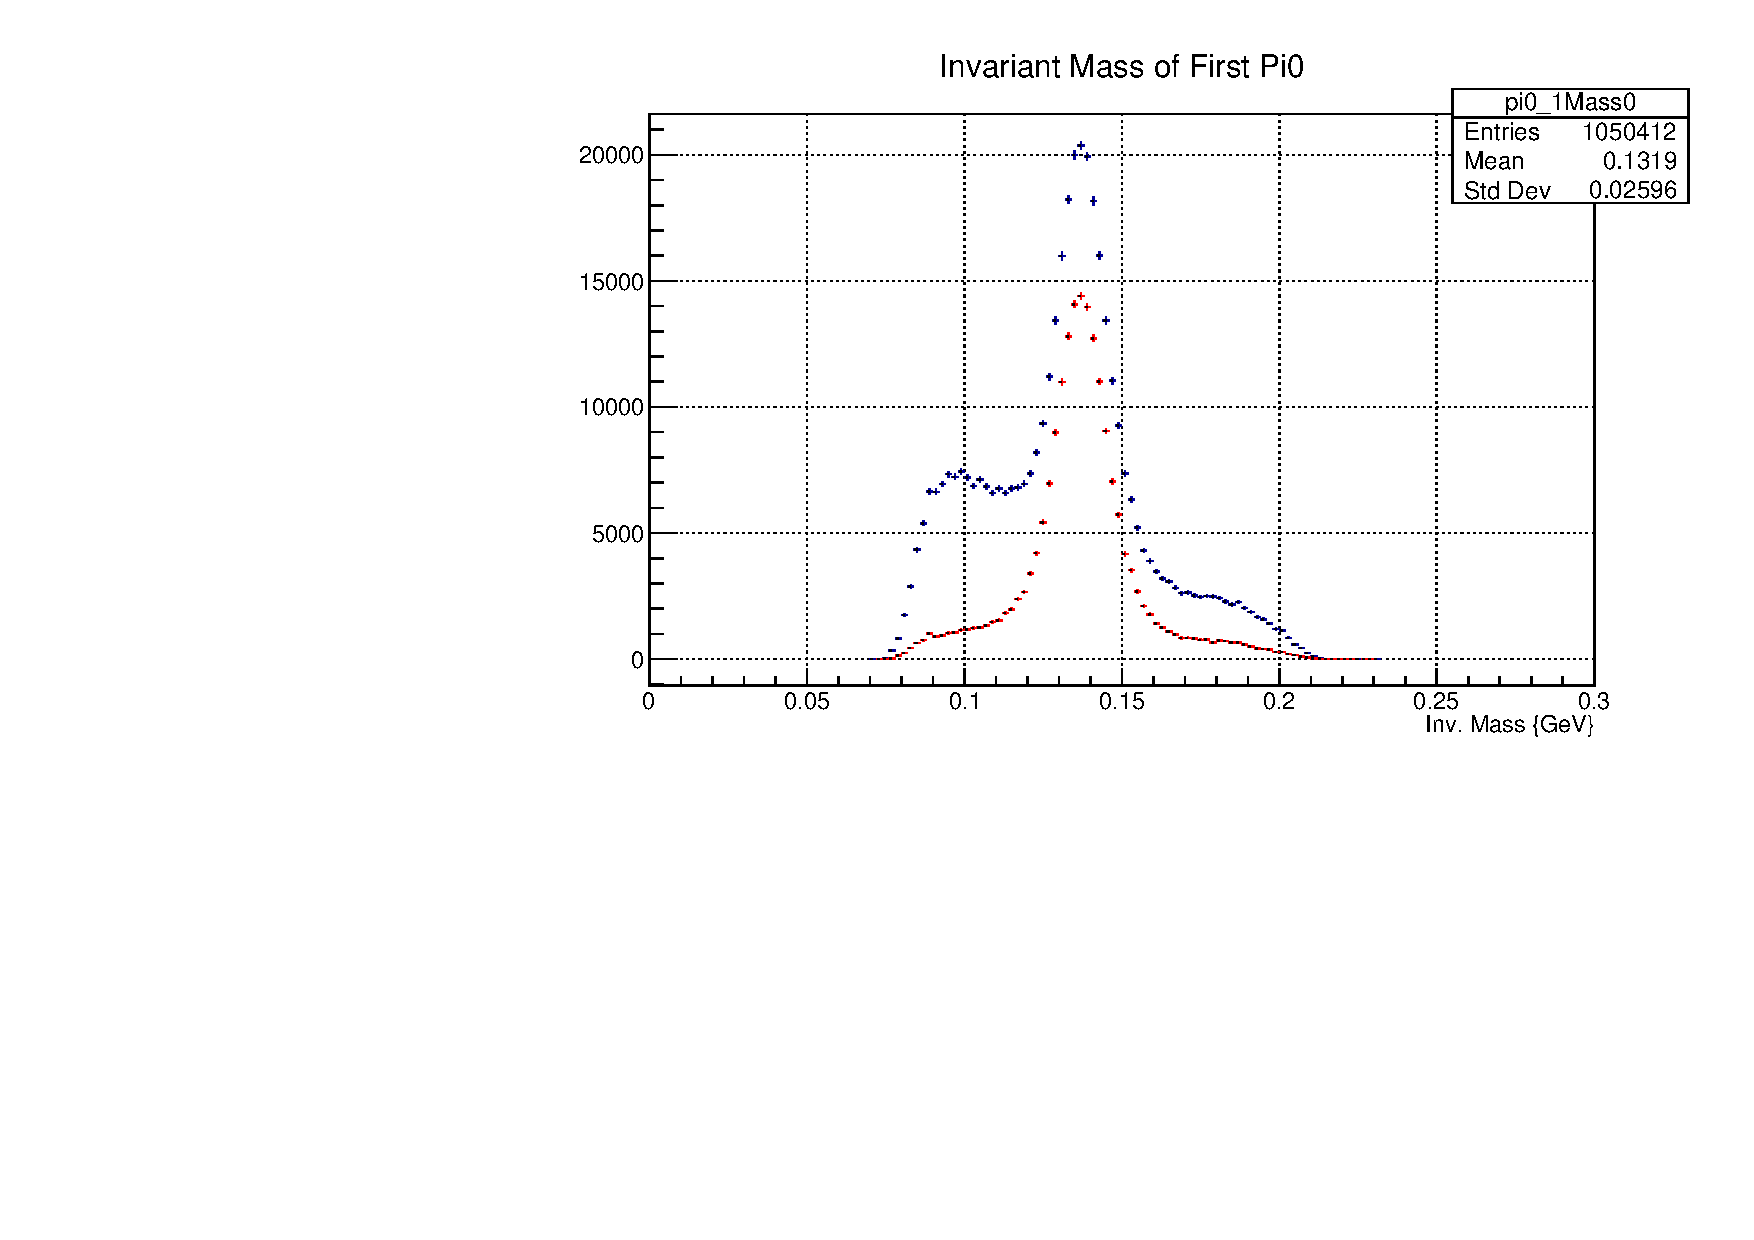
\includegraphics[width=4.75in]{figures/pi0_inv_mass_withpi02cut.pdf}
\caption{Invariant mass of the two photon system with(red) and without(blue) a cut on the invariant mass of the second pair of photons.
\label{fig:pi0yield}}
\end{figure}

These photons are detected by the lead-glass calorimeter and are the
main contribution to the resolution of the reconstructed $\pi^{0}$
mass. A lead-tungstate calorimeter with a substantially better energy
resolution would yield a significant improvement in the signal to
noise ration as the width of the reconstructed $\pi^{0}$ would be
smaller by about a factor of 2.
\subsection{Helium and beryllium targets}
The PrimEx-Eta experiment collected valuable data on light nuclear
targets ($^4$He and $^9$Be) in 2019. Analysis of the two neutral pion
system photoproduction on these nuclei gives a good estimation of the
main background sources, signal to background levels, and the Hall-D
detector resolution for the main kinematic variables of two neutral
pion photoproduction process. The total PrimEx-Eta luminosity
corresponds to approximately one day on
5$\,$\%$\,$rad.$\,$len. beryllium target and 18 days on a
4$\,$\%$\,$rad.$\,$len. helium target at 200$\,$nA electron beam
current and a 10$^{-4}\,$rad.$\,$len. thick amorphous tagger
radiator. The Beryllium target has a thickness of only 1.5$\,$cm
(compare to 30$\,$cm liquid Helium and Hydrogen targets), which allows
constraining interaction point (important for the neutral pions
reconstruction without any additional vertex information from the
tracking system).  First we identified the two neutral pion exclusive
photoproduction process using the energy ratio of two pions to the
initial beam energy with the expected recoil energy
subtracted. Fig.$\,$\ref{fig:pi0elastbe} shows this distribution for
pions detected in FCAL and time accidentals and out-of-target beam
interaction subtracted.
\begin{figure}[!h]
\centering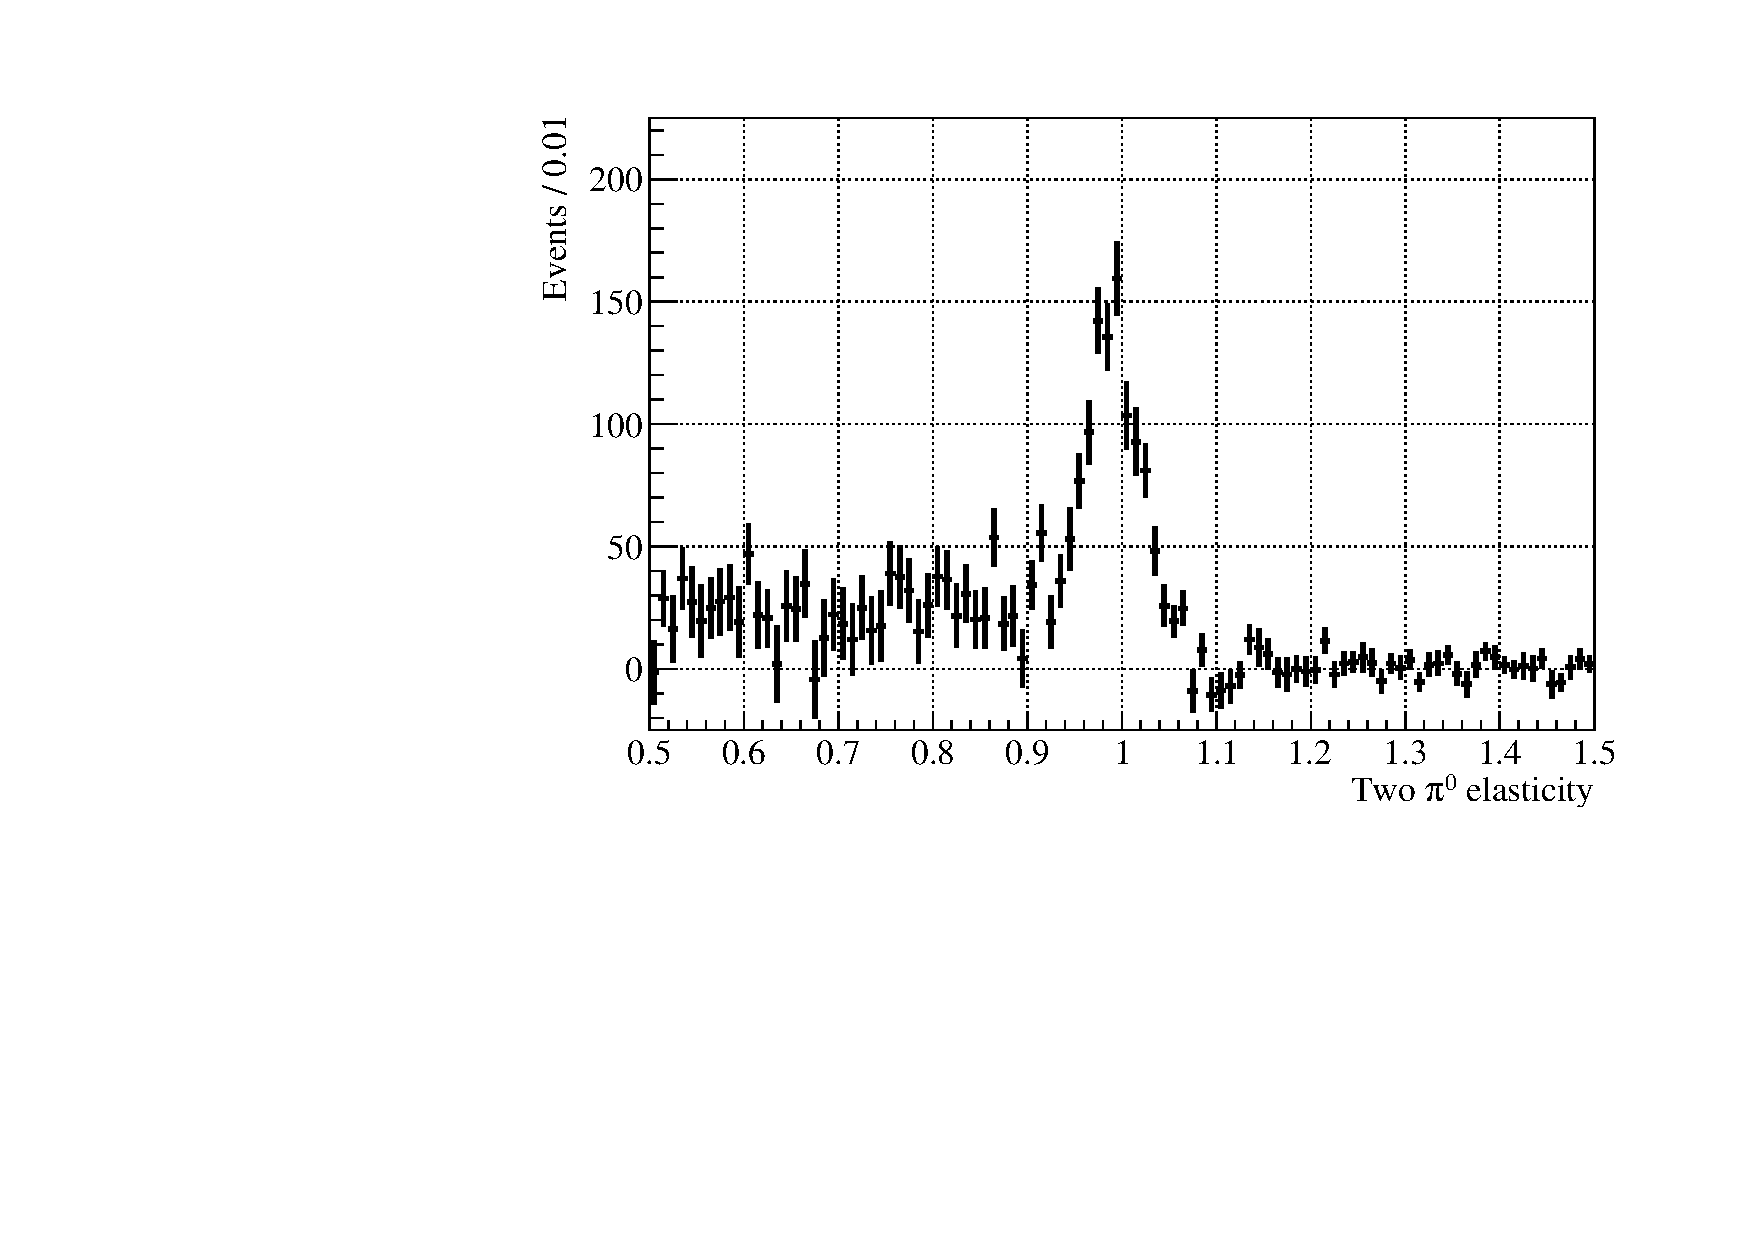
\includegraphics[width=4.75in]{figures/be_elast1.pdf}
\caption{Two neutral pion elasticity (energy ratio to the expected value for the exclusive production) for the Beryllium target.
\label{fig:pi0elastbe}}
\end{figure}
We first required exactly four showers to be detected in FCAL and no
extra showers in BCAL and COMCAL, a minimum shower energy of
0.5$\,$GeV, and no neutral signals in TOF. The number of the signal
events here is about 900, the width of the observed signal with pion
kinematic fit to the mass is about 3$\,$\%, and the signal to
background ratio value is promising. Fig.$\,$\ref{fig:2dbe} shows two
dimensional distribution of those events: elasticity vs invariant
mass. One can see the horizontal line of the exclusive production
events and vertical line of $K_{short}\to\pi^0\pi^0$ decays, which are
separated from each other. Presence of $K_{short}\to\pi^0\pi^0$ decays
in the data is really beneficial for the Primakoff analysis since it
allows tuning the detector resolution in Monte-Carlo and make an
assessment of the level of this value agreement with the data, which
is essential for the successful cross-section fitting procedure and
systematic uncertainty control.
\begin{figure}[!h]
\centering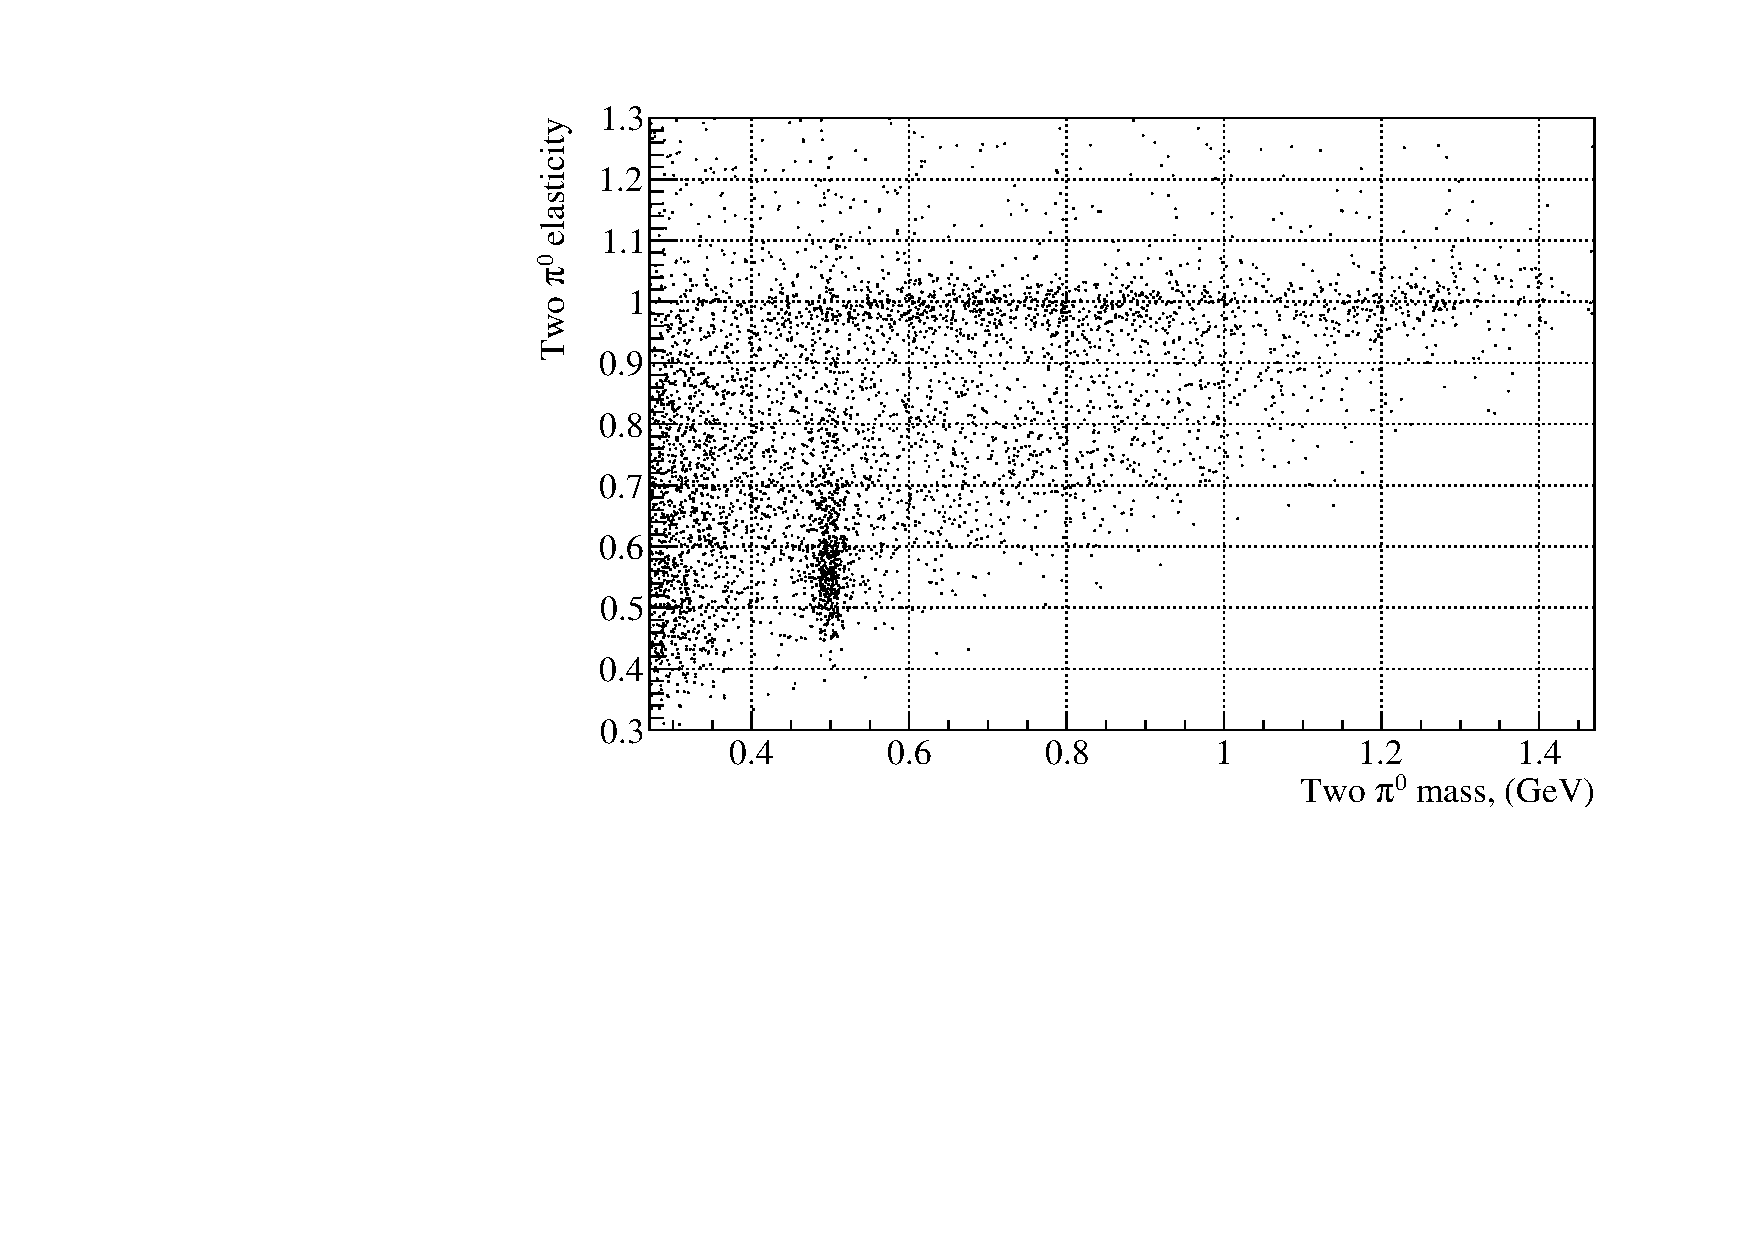
\includegraphics[width=4.75in]{figures/2d_be.pdf}
\caption{Two neutral pion elasticity (energy ratio to the expected value for the exclusive production) vs invariant mass of two pions for the Beryllium target.
\label{fig:2dbe}}
\end{figure}

Including BCAL showers in the neutral pion reconstruction increases
the acceptance (especially for large invariant mass region) and number
of observed events by an order of magnitude. For the beryllium target
this increases the number of exclusive events to $\sim$10$\,$K and for
the helium target to $\sim$200$\,$K events. Fig.$\,$\ref{fig:bemass}
shows two $\pi^0$ invariant mass distribution with the energy within
10$\%$ of the expected for the exclusive production with BCAL included
for low production angle events (below one degree). The $f_2$ meson
peak is clearly seen. Fig.$\,$\ref{fig:beheelast} shows elasticity
distribution for both helium and beryllium targets with BCAL
reconstructions included (time accidentals and ``empty" target
background subtracted).
\begin{figure}[!h]
\centering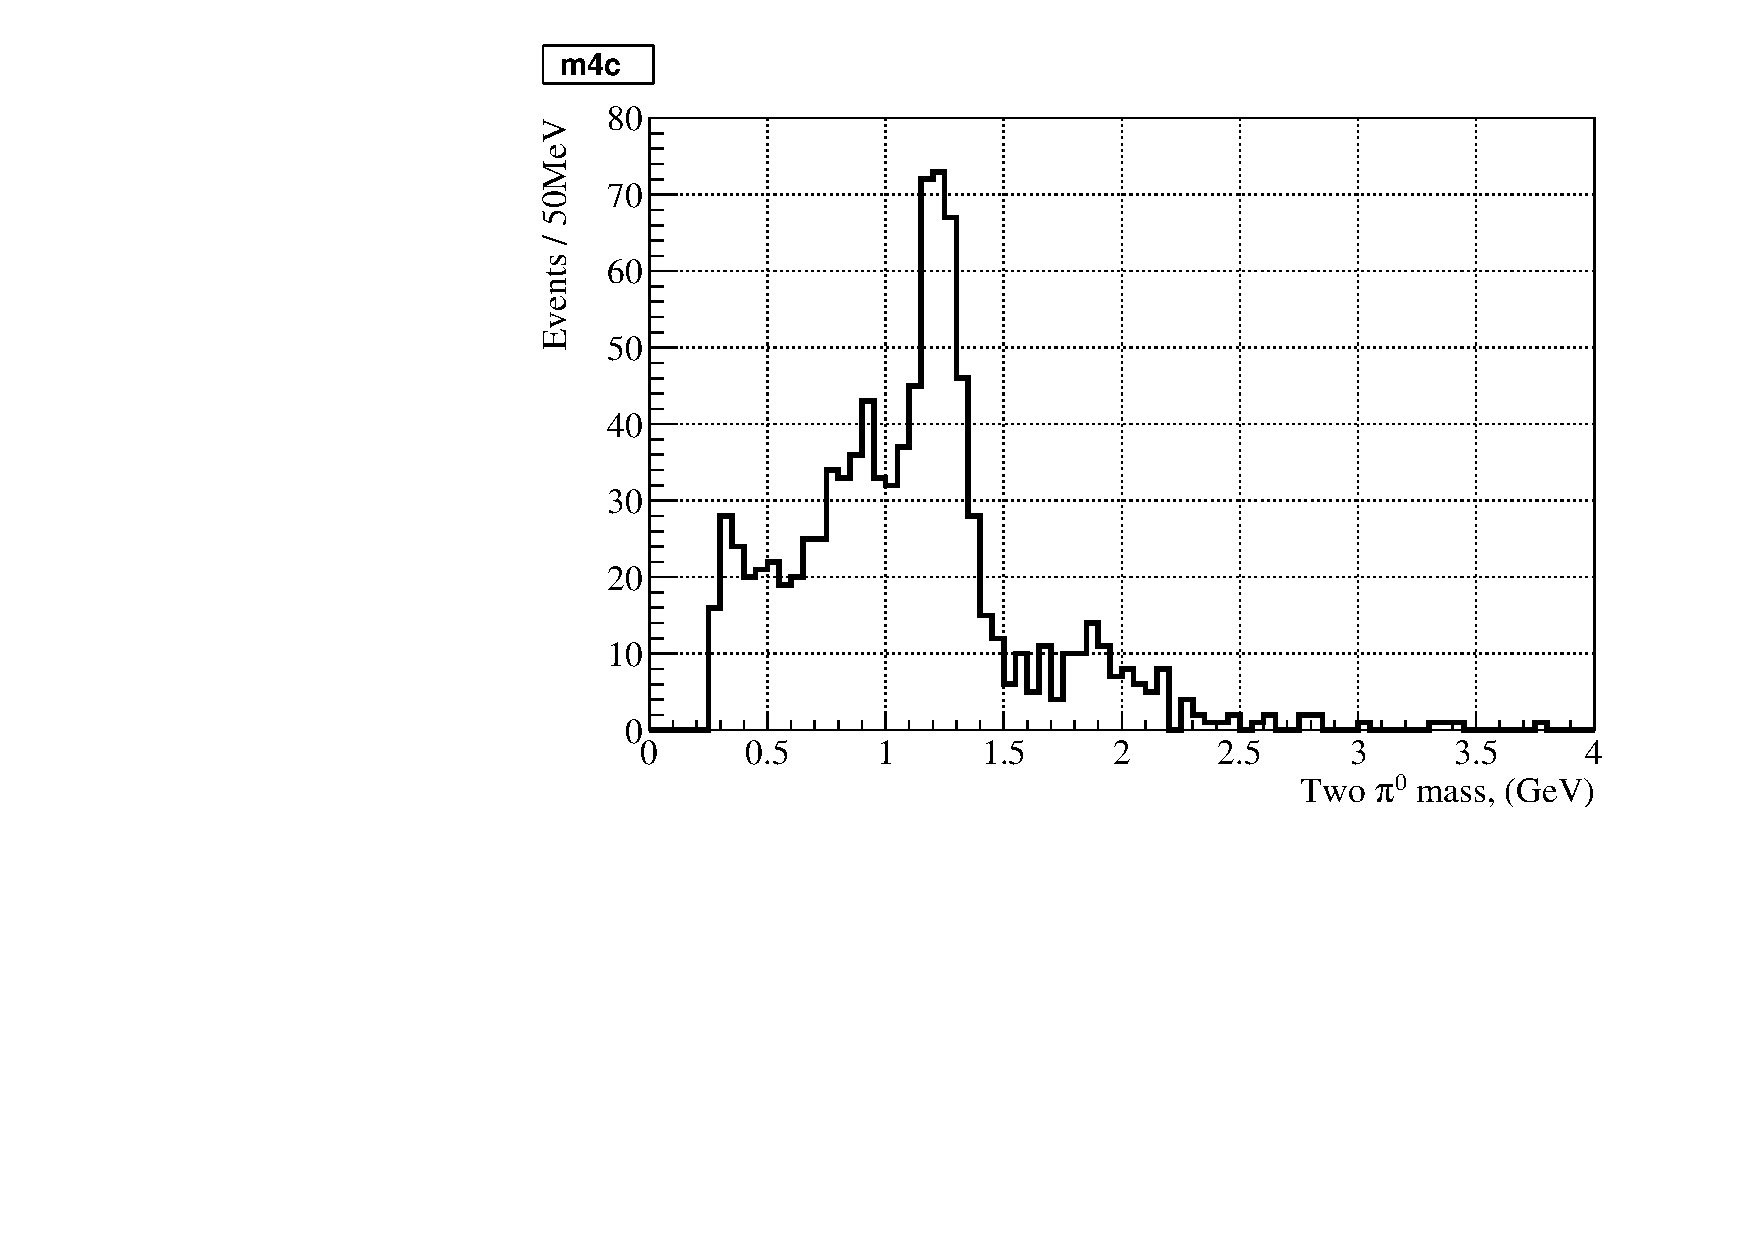
\includegraphics[width=4.75in]{figures/be_mass.pdf}
\caption{Two neutral pion invariant mass for the exclusive events (within 10\% energy), the Beryllium target and production angle below one degree.
\label{fig:bemass}}
\end{figure}
\begin{figure}[!h]
\centering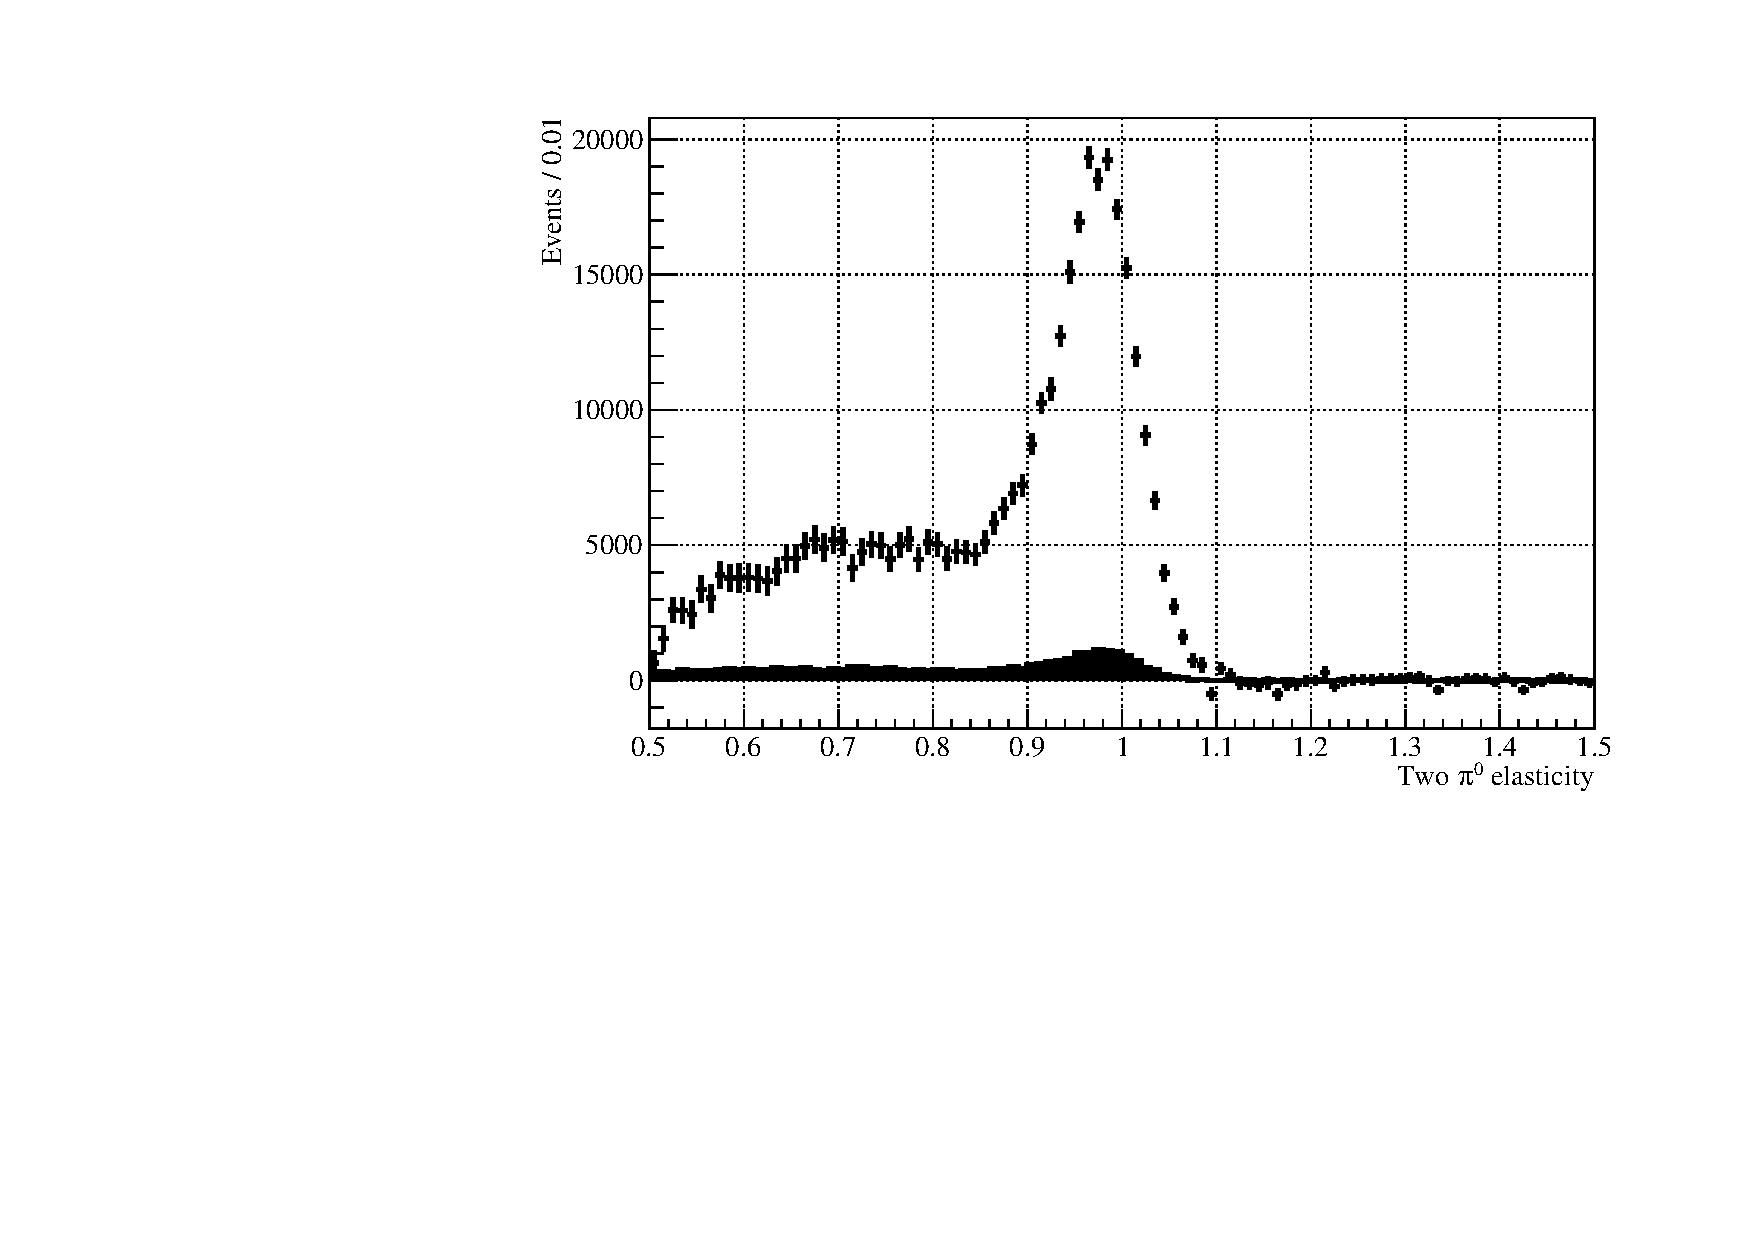
\includegraphics[width=4.5in]{figures/hebe_elast.pdf}
\caption{Two pion elasticity distribution with BCAL included in the analysis. "Empty" target and time accidentals are subtracted. Open histogram - Helium target, $\sim$200$\,$K events in the elastic peak; solid histogram - Beryllium target, $\sim$10$\,$K events in the peak.
\label{fig:beheelast}}
\end{figure}


To conclude this section, we wish to highlight the good detector
resolution for two $\pi^0$ production kinematics variables, the
presence of the calibration process ($K_{short}$) in the data and
controllable level of backgrounds observed for light nuclear targets
exposition.
